
\begin{figure}[ht]
\centering
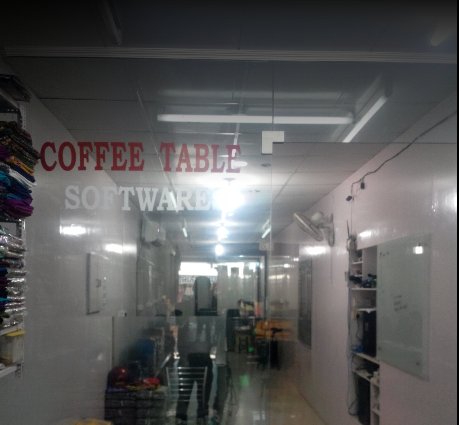
\includegraphics[width=0.6\textwidth]{input/images/coffee.png}
\caption{Coffee Table Softwares Inc.}
\end{figure}
\hspace{-1.7em}
 I had my Internship at Coffee Table Softwares Inc,Ludhiana.
 The firm was started in 2013. There moto is: Our clients are our highest priority. They've worked on a number of platforms and they always prefer using the latest technologies. They've got a great workforce of people who are passionate about everything that they do as a firm. They hold collective responsibility towards their work.\\\\
 Well the name of the firm is Coffee Table Inc, while the website domain is coffeesoftwares.com . They started with such a different yet catchy name. Once you hear it, you'll never forget it. That's for sure. It was taking a lot of caffeine to keep everyone awake for nights while they were setting up everything and so they came up with this idea.\\
The main goal of this firm is:
\begin{itemize}
\item To build and promote their services globally.
\item To promote quality work and undertake projects keeping in view their relevance to needs and requirements of technology in local industry.
\item To work remotely.
\item To build a team and produce great work.
\end{itemize}
Services are being rendered by different pillars of this firm working from different cities like Bangaluru, Ludhiana, Chandigarh etc. mainly in form of expert advice and work in designing, preparation of different business related softwares and many more.\\
Various assignments done by this firm are as follows:

\begin{itemize}
	\item All kind of websites.
	\item Bill cutting softwares with GST feature updates.
	\item Restaurant management system
	\item Home Automation system
	\item Mail server application
	\end{itemize}
\section{Ishwerdas and TCC}

My Training was done by me at Ishwerdas under the guidance of Mr. Inderpreet Singh and I also contributed in projects
made under the guidance of Dr. H.S. Rai at GNDEC,TCC,Ludhiana. \\
At Ishwerdas, they love to create and educate. They believe in creating intelligent interfaces and training inquisitive minds. They help companies, brands and indiviuals build amazing, intelligent apps on web, mobile, desktop and beyond.\\
Few major projects done by Ishwerdas are:
\begin{itemize}
	\item A CRM and Social Community Program (A Circle of Joy)
	\item A javascript based musical website (Replay)
	\item Technical blog that uses Jekyll (Webdioxide.com)

\end{itemize}
 
\begin{figure}[ht]
\centering
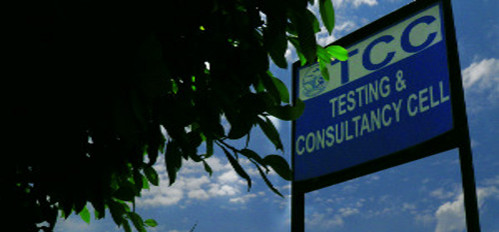
\includegraphics[scale=0.7]{input/images/aw.jpg}
\caption{Testing and Consultancy Cell}
\end{figure}
\hspace{-1.7em} 
TCC-Testing And Consultancy Cell, GNDEC Ludhiana. Guru Nanak Dev Engineering College was established by the Nankana Sahib Education Trust Ludhiana. The Nankana Sahib Education Trust i.e NSET
was founded in memory of the most sacred temple of Sri Nankana Sahib, birth place
of Sri Guru Nanak Dev Ji. With the mission of Removal of Economic Backwardness
through Technology Shiromani Gurudwara Parbandhak Committee i.e SGPC started a
Poly technical was started in 1953 and Guru Nanak Dev Engineering College was established in 1956.\\
Consultancy Services are being rendered by various Departments of the College to the
industry, State Government Departments and Entrepreneurs and are extended in the form of
expert advice in design, testing of materials \& equipment, technical surveys, technical audit,
calibration of instruments, preparation of technical feasibility reports etc. \\\\
It was established in the year 1979 with a basic aim to produce
quality service for technical problems at reasonable and affordable rates as a service to society
in general and Engineering fraternity in particular.\\
This consultancy cell of the college has given a new dimension to the development
programmers of the College. Consultancy projects of over Rs. one crore are completed by the
Consultancy cell during financial year 2009-10. \\\\
Various Major Clients of the Consultancy Cell are as under:

\begin{itemize}
\item Northern Railway, Govt. of India
\item Indian Oil Corporation Ltd.
\item Larson \& Turbo.
\item Multi National Companies like AFCON \& PAULINGS.
\item Punjab Water Supply \& Sewage Board
\item Power Grid Corporation of India.
\item National Building Construction Co.
\item Punjab State Electricity Board.
\item Punjab Mandi Board.
\item Punjab Police Housing Corporation.
\item National Fertilizers Ltd.
\item GLADA, Ludhiana
\end{itemize}


